The experiment was carried out on ten healthy subjects, two women and eight men, nine right-handed and one left-handed, that participated voluntarily in the experiment.

They were prepared to the experiment by placing on their dominant arm seven single-differential Aurion ZeroWire wireless electrodes for surface EMG and by giving them a force sensor (FUTEK LMD500 Hand Gripper) in order to detect the force exerted during the grasp (Figure~\ref{fig:SubjSetup}); they were given no knowledge of what the experiment was.

\begin{figure*}[!t] \centering
  \begin{tabular}{ccc}
   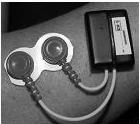
\includegraphics[height=0.16\textheight]{figs/Electrode} &
    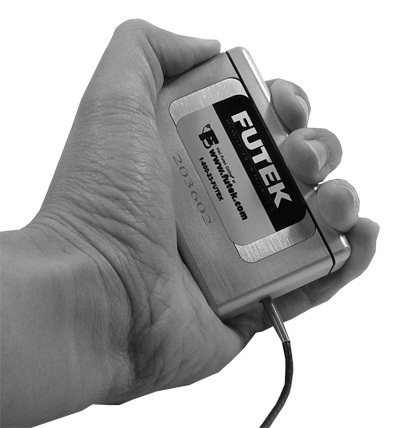
\includegraphics[height=0.16\textheight]{figs/Hand_Gripper} &
    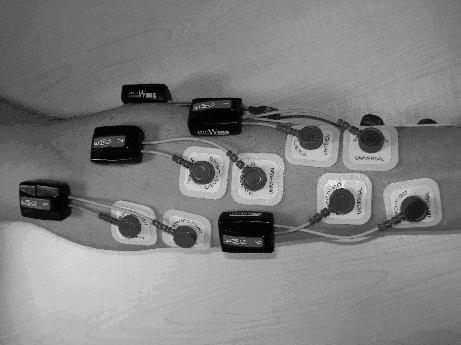
\includegraphics[height=0.16\textheight]{figs/El_Arrangement} \\
    $(a)$ & $(b)$ & $(c)$ \\
  \end{tabular}
  \caption{The experimental setup (\textit{subject side}): (a) An EMG wireless electrode; (b) The FUTEK hand gripper sensor; (c) The arrangement of the electrodes on the ventral side of the subject's arm.}
  \label{fig:SubjSetup}
\end{figure*}

At the same time, the experimenter desk was equipped with a National Instruments data acquisition board (NI-USB6211) connected to the receiver of the EMG wireless device and to the Weathstone bridge circuit of the Hand Gripper amplifier (Figure~\ref{fig:ExpSetup}). The board's cable was plugged into the USB port of a laptop computer.
These connections makes the PC acquire simultaneously all the data through a custom LabView VI.
  
\begin{figure*}[!t] \centering
  \begin{tabular}{cc}
   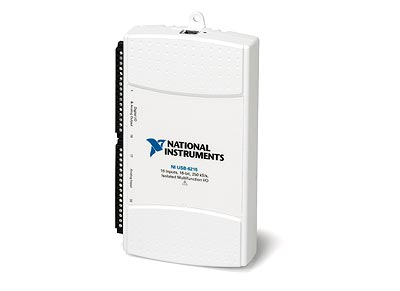
\includegraphics[height=0.16\textheight]{figs/NI-6211} &
    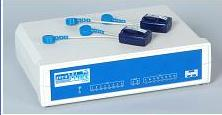
\includegraphics[height=0.16\textheight]{figs/Zero_Base} \\
  $(a)$ & $(b)$\\
  \end{tabular}
  \caption{The experimental setup (\textit{experimenter side}): (a) The USB data acquisition card (NI-USB6211). (b) The EMG device receiver.}
  \label{fig:ExpSetup}
\end{figure*}

The electrodes were positioned, according to the medical literature, as carefully as possible in order to identify the best EMG sources and to detect the activity of the most relevant flexor and extensor muscles of the forearm. The signals coming from the EMG device and from the FUTEK load cell were sampled at 2 KHz.

The experiment was made by two phases following one after the other. During the first one, the subject had his arm still and relaxed on a table; in this condition, he was asked to grasp the sensor using, in turn, three different grips (Figure~\ref{fig:Grasps}):
\begin{itemize}
	\item index precision grip;
	\item other fingers precision grip;
	\item power grasp.
\end{itemize}

\begin{figure*}[!t] \centering
  \begin{tabular}{ccc}
   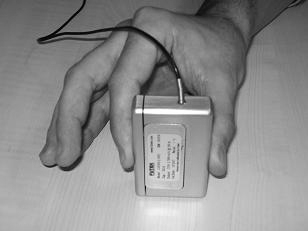
\includegraphics[height=0.16\textheight]{figs/grip1} &
    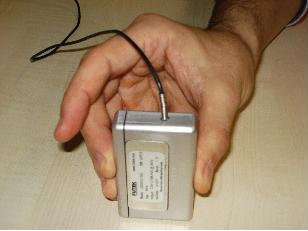
\includegraphics[height=0.16\textheight]{figs/grip2} &
    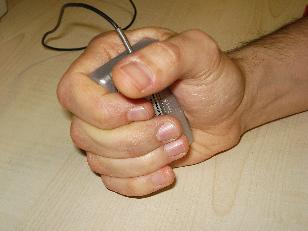
\includegraphics[height=0.16\textheight]{figs/grip3} \\
    $(a)$ & $(b)$ & $(c)$ \\
  \end{tabular}
  \caption{The three different grasps: (a) Index precision grip. (b) Other fingers precision grip. (c) Power grasp.}
  \label{fig:Grasps}
\end{figure*}

A rest condition was sampled beforehand to define the baseline of the emg activity of each muscle.

The subject freely repeated each grasping action for 100'', resting for 30'' in between grasps. The whole procedure was repeated twice, in order to gather more data and diminish the effect of local, statistically irrelevant, errors. 
Since now, this phase will be referred to as \emph{Still-Arm experiment (SA)}.

A second phase, actually the more interesting one for the final intent of this study, consisted in repeating the same exercise in a less severe condition. The subject was asked to grasp the \textit{hand gripper} while he was freely moving, walking around, lifting and pronating/supinating his arm and forearm; this choice, to emulate the main movements that one is expected to do during his DLAs.
This second phase was called \emph{Free-Arm experiment (FA)}.


As a whole, each subject's experiment resulted in something more than 1200'' of data. At first, this amount of data was pre-processed, subject by subject, by evaluating the \emph{Root Mean Square (RMS)} of the EMG signal over a certain time-window; then they were reduced via an \emph{Online Uniformisation (OU)}.

The Root Mean Square (also known as the Quadratic Mean) is a statistical measure of the magnitude of a varying quantity. It is well-known to make the EMG signal highly related to the muscular force.

\begin{displaymath}
x_{rms} = \sqrt{\frac{1}{n}\sum_{i=1}^{n}x_{i}^{2}}
\end{displaymath}

In a certain way, the RMS acts like a low-pass filter that smooths the high frequency components of the signal by averaging them with the lower ones.
Moreover, even though the RMS is affected by a phase error that depends on the length of the window (n), this error is supposed to be useful for the analysis of the relationship between EMG and exerted force because it partially compensates the EMG-to-movement latency.

The second step, the Online Uniformisation, is required in order to reduce properly, i.e. without over-degrading its performance, the number of samples that are passed to the machine learning system in order to make it usable for real-time applications; this is actually the medium-term aim of this work.

To do that, the Online Uniformisation algorithm discards any samples that are too close to other samples that have been already acquired, according to Euclidean distance.

During the analysis, a grid search on different RMS window lengths and different Online Uniformisation distances has been performed to identify the values that produce respectively the best classification and regression results.

Subsequently two different implementations of the Support Vector Machines theory that uses a Gaussian kernel model were employed to:
\begin{itemize}
	\item map the connection between the EMG signal and the type of grasp (\textit{classification});
	\item estimate the force applied to the force sensor (\textit{regression}).
\end{itemize}

\begin{figure*}[!t] \centering
  \begin{tabular}{c}
    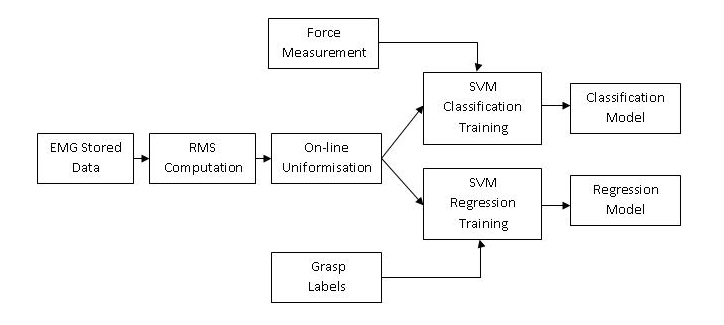
\includegraphics[height=0.3\textheight]{figs/Schema} \\
  \end{tabular}
  \caption{Processing algorithm.}
  \label{fig:Algorithm}
\end{figure*}
